% 3. Data Corpus and Preprocessing Methodology
\section{The Need for Unification}
\label{ch:unitraj}

This section presents an overview of the need for a unified framework for trajectory prediction in autonomous driving, addressing the challenges of dataset heterogeneity and the complexities of motion forecasting tasks. The discussion highlights the importance of standardizing data formats, feature characteristics, and preprocessing pipelines to enable effective model training and evaluation across diverse datasets.

\subsection{Unification of Motion Forecasting Datasets}
\label{sec:data_datasets}

The \texttt{UniTraj} framework addresses the fundamental challenge of standardizing multiple motion-forecasting datasets that exhibit substantial heterogeneities in both \emph{data formats} and \emph{feature characteristics}.
The former encompasses differences in data structure and organization, while the latter stems from variations in
spatio-temporal resolution, coverage range, and semantic annotation schemes.

To overcome format discrepancies, \texttt{UniTraj} leverages \texttt{ScenarioNet}~\cite{scenarionetLi2023} for conversion into a common
format, thereby eliminating the need for multiple preprocessing implementations. However, feature characteristics require additional harmonization. Temporal coverage varies substantially
across datasets, with historical trajectories ranging from 1 second in \texttt{WOMD}\cite{wmodSun2020} to 5 seconds in \texttt{Argoverse 2}\cite{av2Wilson2023},
and future prediction horizons extending from 6 to 8 seconds. Map resolutions and semantic annotations differ
significantly, with all datasets providing \emph{scene-centric} HD maps at varying resolutions.
Agent features also exhibit substantial variations: \texttt{nuScenes} provides only velocity and heading, while
\texttt{WOMD} includes comprehensive 3D bounding box annotations. Notably, \texttt{Argoverse 2} provides bounding
box and rich semantic annotations, but these are lost during \texttt{ScenarioNet} format conversion.
The conversion and normalization process is outlined in~\autoref{ssec:data_pipeline}.

\subsection{Unified ML Infrastructure}
Beyond dataset unification, trajectory prediction research requires a comprehensive machine learning infrastructure that handles the complexities of modern deep learning workflows. The UniTraj framework addresses this need by providing essential components that allow researchers to focus on model innovation rather than infrastructure implementation.

These components encompass the complete research pipeline: training and evaluation frameworks, data handling and preprocessing modules, logging and visualization tools, shared metrics and loss functions, and experiment management systems that facilitate reproducibility and systematic experimentation. Such a framework should be designed with transparency and modularity as core principles, enabling seamless extension and integration of new datasets, models, evaluation metrics, and additional functionalities such as callbacks or custom training procedures.



\subsection{Limitations of UniTraj}
\label{sec:data_challenges}

While the original UniTraj framework provided foundational functionality for unified trajectory prediction research, it suffered from poor software quality and architectural design, which limited its usability and transparency. As the goal of this seminar work was to understand the task of motion forecasting from the ground up, we undertook a comprehensive refactoring of the UniTraj framework to address these limitations in order to achieve a holistic understanding of components belonging to the motion forecasting task.

Some of the most significant limitations of the original UniTraj framework, that motivated the refactoring, are summarized below:

\begin{itemize}[leftmargin=*]
    \item \textbf{Monolithic Architecture:} The complex data processing pipeline consisted of a single monolithic script with poor separation of concerns, making it almost impossible to understand data flow and transformations, extend individual components or fix issues that we observed in the resulting dataset.
    \item \textbf{Insufficient Type Safety:} Critical symbols lacked proper type hints, comments, and docstrings; the \texttt{Hydra} configuration system was used as an untyped dictionary without structural validation, such that it was difficult to work with these configuration objects, to understand the impact or expected values of parameters, and to catch potential issues early in the development process.
    \item \textbf{Data Split Integrity:} The framework failed to respect original train/validation/test splits from source datasets, violating standard machine learning practices. Our efforts to resolve this issue turned out to be quit frustrating due to the intransparent path and file handling in the original implementation.
    \item \textbf{Inadequate Documentation:} Absence of comprehensive documentation and standardized coding practices made it challenging to work with and understand the framework.
\end{itemize}

\paragraph{Infrastructure and Framework Integration Issues.}
Despite utilizing modern frameworks like PyTorch Lightning, the implementation failed to follow recommended practices:

\begin{itemize}[leftmargin=*]
    \item \textbf{PyTorch Lightning Misuse:} Improper integration lacking \texttt{LightningDataModule} usage, inadequate logging functionality, no easy configuration of the components of this framework and improper integration with Weights \& Biases.
    \item \textbf{Path Management Deficiencies:} Poor filesystem path handling without clear control over data sources, destinations, model checkpoints, and logs.
    \item \textbf{Missing Training Capabilities:} Absence of essential deep learning features including automatic mixed precision, gradient accumulation, learning rate scheduling, distributed computing support, and essential callbacks (learning rate monitors, early stopping, model checkpointing), all of which are relatively easy to use if PyTorch Lightning is used properly.
\end{itemize}


\subsubsection{Revision of the UniTraj Framework}
This section details the comprehensive refactoring applied to the original UniTraj framework to achieve a modular, type-safe, and extensible codebase that addresses all identified limitations while maintaining full functionality.\\
The revised framework implements a hierarchical configuration-driven architecture, of which a small subset is visualized in Figure~\ref{fig:unitraj_data_architecture}.

\begin{figure}[htbp]
    \centering
    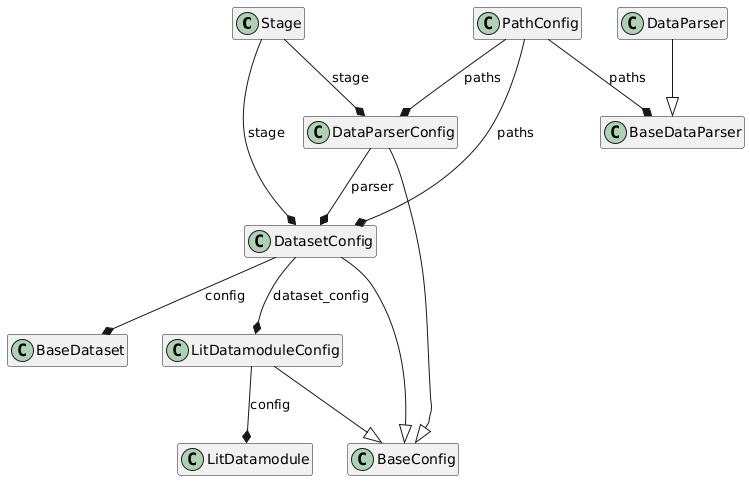
\includegraphics[width=0.9\textwidth]{figures/classes_DataHandling.png}
    \caption{UniTraj data handling architecture showing the relationships between configuration classes, data parsers, datasets, and Lightning modules.}
    \label{fig:unitraj_data_architecture}
\end{figure}

\paragraph{Core Architectural Improvements.}
The refactoring introduced three foundational design patterns that address the primary limitations of the original implementation:

\begin{itemize}[leftmargin=*]
    \item \textbf{Config-as-Factory Pattern:} Implemented through \href{https://github.com/JanDuchscherer104/UniTraj/blob/main/unitraj/utils/base_config.py}{\texttt{BaseConfig}} with strongly typed configuration classes for each functional component. Every configuration object serves as both a type-safe parameter container and a factory for instantiating its corresponding component.

    \item \textbf{Modular Data Processing Pipeline:} Decomposed the monolithic preprocessing script into three specialized stages with clear separation of concerns: \href{https://github.com/JanDuchscherer104/UniTraj/blob/main/unitraj/datasets/base_dataparser.py}{\texttt{BaseDataParser}} orchestrates high-level pipeline execution including multiprocessing, HDF5 storage, and metadata collection; \href{https://github.com/JanDuchscherer104/UniTraj/blob/main/unitraj/datasets/dataparser.py}{\texttt{DataParser}} implements a nine-phase preprocessing pipeline; and \href{https://github.com/JanDuchscherer104/UniTraj/blob/main/unitraj/datasets/base_dataset.py}{\texttt{BaseDataset}} provides efficient PyTorch-compatible data loading.

    \item \textbf{Strongly Typed Interfaces:} Introduced comprehensive type definitions in \href{https://github.com/JanDuchscherer104/UniTraj/blob/main/unitraj/datasets/types.py}{\texttt{types.py}} using \texttt{TypedDict} and Pydantic \texttt{BaseModel} classes, replacing untyped dictionary passing and enabling compile-time shape validation. Defines \texttt{RawScenarioDict}, \texttt{ProcessedDataDict}, \texttt{DatasetItem}, and \texttt{BatchInputDict} interfaces.
    \item \textbf{Lightning Data Module:} \href{https://github.com/JanDuchscherer104/UniTraj/blob/main/unitraj/lightning/lit_datamodule.py}{\texttt{LitDatamodule}} provides standardized data loading with custom collate functions, configurable batch sizes, worker processes, and automatic train/validation/test split handling while maintaining original dataset split integrity.
    \item \textbf{Trainer Factory:} \href{https://github.com/JanDuchscherer104/UniTraj/blob/main/unitraj/lightning/lit_trainer_factory.py}{\texttt{LitTrainerFactory}} enables easy \texttt{pl.Trainer} configuration with support for multi-GPU training, mixed precision, gradient accumulation, learning rate scheduling, and comprehensive callback management.
\end{itemize}

\paragraph{Infrastructure and Monitoring Enhancements.}
Comprehensive improvements to logging, experiment tracking, and development workflows:

\begin{itemize}[leftmargin=*]
    \item \textbf{Centralized Path Management:} \href{https://github.com/JanDuchscherer104/UniTraj/blob/main/unitraj/configs/path_config.py}{\texttt{PathConfig}} consolidates all filesystem paths with automatic directory creation and propagation to child configurations, eliminating scattered path management errors.

    \item \textbf{Hierarchical Configuration:} The \href{https://github.com/JanDuchscherer104/UniTraj/blob/main/unitraj/configs/experiment_config.py}{\texttt{ExperimentConfig}} serves as the top-level orchestrator with automatic parameter propagation and the \texttt{inspect()} method for complete configuration tree visualization, improving experiment reproducibility.

    \item \textbf{Experiment Tracking:} Integrated \href{https://github.com/JanDuchscherer104/UniTraj/blob/main/unitraj/configs/wandb_config.py}{\texttt{WandBConfig}} provides comprehensive experiment tracking with real-time metric logging, hyperparameter sweeps, and model artifact management.

    \item \textbf{Type Safety and Validation:} Added precise type annotations throughout the codebase, enabling \texttt{mypy} enforcement and Pydantic validation for all configuration objects, catching potential runtime errors at development time.
\end{itemize}

Further relevant components can be found in the directory tree in~\autoref{app:directory_structure}.

\newpage